\documentclass{acmsiggraph}
%\documentclass[review]{acmsiggraph}

\TOGonlineid{paper1037} %TODO

\setlength{\ACMcopyrightspace}{1.0in}


%\title{A Polyfill Approach to Declarative Integration of Interactive 3D Graphics\\ into the World-Wide Web}
\title{Declarative Integration of Interactive 3D Graphics into the World-Wide Web:\\Principles, Current Approaches, and Research Agenda}


\author{
Jacek Jankowski\thanks{e-mail:jacek.jankowski@inria.fr} \\ Inria \\ Bordeaux \\ France
\and Sandy Ressler\thanks{e-mail:sandynist@gmail.com} \\ NIST \\ Gaithersburg MD \\ USA
\and Kristian Sons\thanks{e-mail:kristian.sons@dfki.de} \\ DFKI \\ Saarbr\"ucken \\ Germany
\and Yvonne Jung\thanks{e-mail:yvonne.jung@igd.fraunhofer.de} \\ Fraunhofer IGD \\ Darmstadt \\ Germany
\and Johannes Behr\thanks{e-mail:johannes.behr@igd.fraunhofer.de} \\ Fraunhofer IGD \\ Darmstadt \\ Germany
\and Philipp Slusallek\thanks{e-mail:slusallek@cs.uni-saarland.de} \\ DFKI \& Saarland University \\ Saarbr\"ucken \\ Germany
}

\pdfauthor{Jacek Jankowski, Sandy Ressler, Kristian Sons, Yvonne Jung, Johannes Behr, Philipp Slusallek}

\keywords{Declarative 3D, HTML5, DOM Integration, Polyfill}


\begin{document}

\maketitle

\begin{abstract}
With the advent of WebGL, plugin-free hardware-accelerated interactive 3D graphics has finally arrived in all major Web browsers.
WebGL is an imperative solution that is tied to the functionality of rasterization APIs. Consequently, its usage requires a deeper understanding of the rasterization pipeline. In contrast to this stands a declarative approach with an abstract description of the 3D scene. We strongly believe that such approach is more suitable for the integration of 3D into HTML5 and related Web technologies, as those concepts are well-known by millions of Web developers and therefore crucial for the fast adoption of 3D on the Web.
Hence, in this paper we explore the options for new declarative ways of incorporating 3D graphics directly into HTML to enable its use on any Web page. We present declarative 3D principles that guide the work of the \textit{Declarative 3D for the Web Architecture W3C Community Group} and describe the current state of the fundamentals to this initiative. Finally, we draw an agenda for the next development stages of Declarative 3D for the Web.
\end{abstract}

\begin{CRcatlist}
  \CRcat{I.3.7}{Computer Graphics}{Three-Dimensional Graphics and Realism}{Virtual Reality}
  \CRcat{I.3.6}{Methodology and Techniques}{Standards}{Languages}
\end{CRcatlist}

\keywordlist

\copyrightspace


\section{Introduction}

The Web evolved from a text-based system to the current rich and interactive medium that supports images, 2D graphics, audio and video. These types of new media have made the Web experience richer, more attractive to users, etc, than ever before, and opened up possibilities for new types of applications and usage. The major media type that is still missing is 3D: synthetic, possibly photorealistic images in 3D with animation, as smoothly integrated in the everyday Web experience as images or video. Just as the appearance of images or video could open new application possibilities, access to the 3D on a Web site would make it possible to include realistic models of 3D objects -- from models of buildings to representation of the human body or the sceneries for computer games. With WebGL \cite{WebGL12}, a JavaScript binding for OpenGL ES 2.0, this seems feasible; however, the goal would be to achieve the same smooth inclusion of 3D content in a Web page like we experience today with images or SVG-based 2D graphics.

Although some of these goals could also be achieved by imperative means (e.g., through the usage of WebGL), developments of 3D models have a long tradition of using declarative approaches, which is also in line with some of the fundamental principles of Web development. It is therefore important to explore how the experiences accumulated in two different communities, namely the Web Development and Computer Graphics communities, can be capitalized upon to achieve the long term goal of using 3D on the Web the same way as we do with 2D graphics and video today.
Moreover, while imperative graphics APIs are powerful and necessary, a \emph{Declarative 3D} approach can provide web authors an easy way to add interactive high-level declarative 3D objects through the HTML Document Object Model (DOM) allowing them to easily create, modify, share, and experience interactive 3D graphics using HTML documents. Figure \ref{fig:DeclarativeVsImperative} depicts the position of the Declarative 3D approach in the current Web graphics technology ecosystem.

\begin{figure}%[ht]
  \centering
  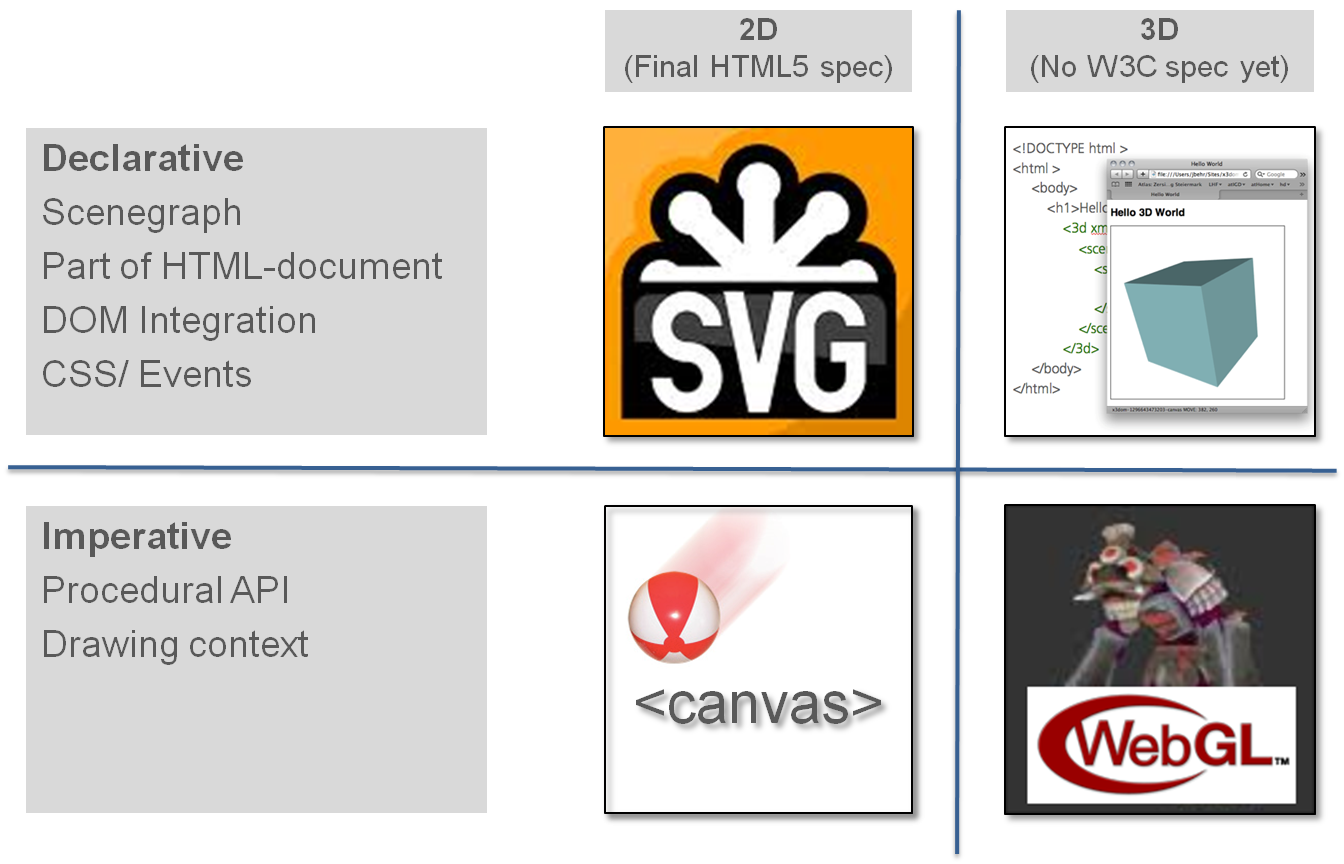
\includegraphics[width=1.0\columnwidth]{images/Declarative3d.png}
  \caption{The position of the Declarative 3D approach in the current Web graphics technology ecosystem.}
  \label{fig:DeclarativeVsImperative}
  %\vspace{-0.2cm}
\end{figure}

It is arguable that the emerging support for an imperative 3D API for the Web is useful but insufficient for broad acceptance and usage of 3D on the Web. A declarative approach that offers qualified concepts and that is tightly integrated with current web technologies, such as JSON or XML for scene construction, DOM for scene manipulation, and CSS for styling, is necessary to support a fast adoption and broad use of interactive 3D graphics by the millions of Web developers. The provided concepts must lift the hardware-oriented imperative application programming interfaces to an expressive and more easily usable level. Therefore not the low-level data structures of existing GPU layers must be in the center of the design but high-level elements and items like 3D objects, transformations, material descriptions, and lights. Instead of teaching Web developers 3D graphics APIs, the goal is to bring 3D graphics to the point where it is natural for Web developers to just make use of it. While this might not be possible for every possible use of a low-level API, it still can cover the vast majority of use cases.

The \textit{Declarative 3D for the Web Architecture W3C Community Group} (Dec3D) \cite{Dec3D} was thus founded to suggest and create methods to add high-level declarative 3D objects to the HTML DOM \cite{W3C-DOM}, so users can share and experience interactive 3D contents. Moreover, this not only allows creating new content from existing content but also to index and search 3D content.
The core mission is to determine the requirements, options, and use cases for the integration of interactive 3D graphics into the Web technology stack in a declarative way, which hopefully will provide a foundation for future standardization.
Therefore, the group aims at presenting common use cases that define how 3D might intersect and interact with HTML5, DOM events, CSS, SVG, GeoLocation, Augmented Reality, Efficient XML Interchange (EXI) \cite{EXI} and other key working groups, whereas certain complex data types (e.g., transformation matrices) and computations are also of mutual interest. In this regard, this paper presents the current state and efforts concerning Dec3D.

\begin{figure*}%[ht]
  \centering
  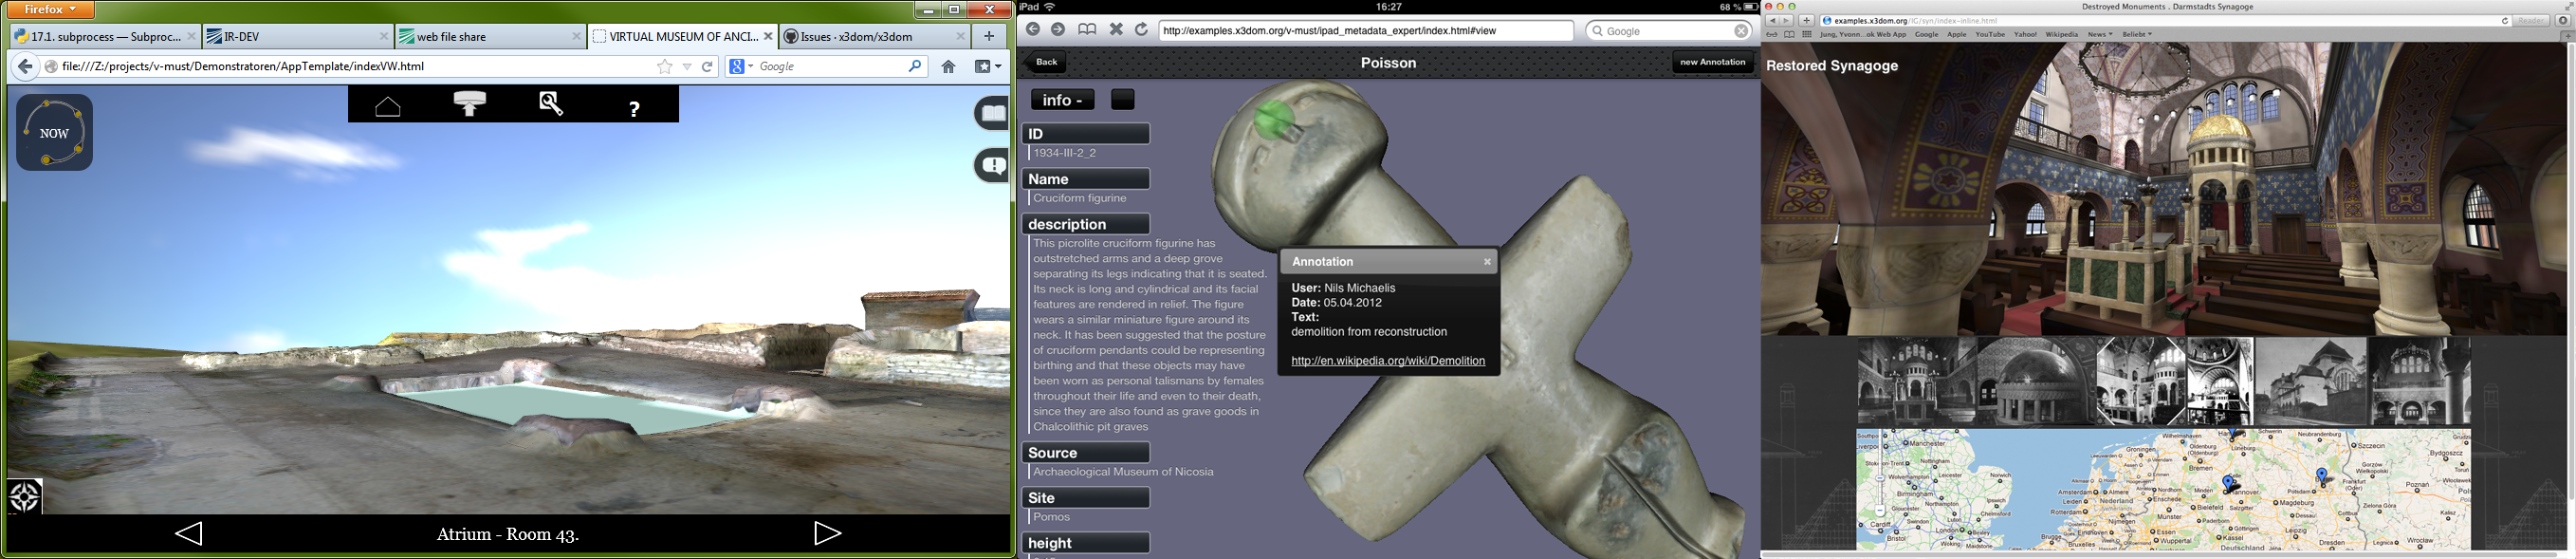
\includegraphics[width=1.0\textwidth]{images/ch_apps.png}
  \caption{From left to right: walktrough of Roman heritage site; cultural heritage object explorer with metadata; restored virtual synagoge.}
  \label{fig:chApps}
  %\vspace{-0.2cm}
\end{figure*}



\section{Declarative 3D Principles}
\label{sec:Principles}

Here we describe declarative 3D principles, where the following goals should guide the development of DOM-based 3D graphics.

\paragraph{Following the Established Principles of the Web}
Declarative 3D is being developed to significantly lower the barrier for authoring 3D content for Web sites by duplicating the key features that enabled the growth of the early Web and its further success.

\begin{description}
  \item [Separation of structure from content] Underlying the Web from its earliest days was the separation of structure from content. The concept of a paragraph specified by the \verb|<p>| tag was separate from its content. Declarative 3D is attempting to bring the same separation to 3D graphics inside of web pages. The concepts such as definitions of 3D objects, transformations, materials, etc. should be implemented in a declarative 3D description as an extension to HTML5 \cite{HTML5} using any existing or future extension mechanism.
  \item [Separation of content from style] One of the principles of the current Web is also the separation of content and style, most notably through CSS. The successful integration of SVG \cite{svg} with HTML was made much easier due to the fact that SVG was already following this principle. The objective here is to extend the use of CSS for styling 3D graphics. One example can be the use of the latest CSS3 3D Transforms \cite{webkit3DCSS} to allow manipulating not only 2D but also 3D objects.
  \item [Use of the Document Object Model] The DOM \cite{W3C-DOM} is a platform- and language-neutral interface that allows programs and scripts to dynamically access and update the content, structure and style of Web documents. Declarative 3D should use the DOM API to examine and modify elements on the 3D scene and their attributes by simply reading and setting their properties. As the DOM provides access to user actions (e.g., pressing a key or clicking a mouse button), it should also be used as a main interface to interact with 3D contents.
\end{description}

Embedded 3D graphics should reuse existing W3C techniques, specifically from HTML5 and SVG, as far as possible and propose extensions only where specific features are necessary or provide significant benefits. Where new concepts are introduced their relation to and effects on existing Web standards should be analyzed, evaluated, and discussed with the respective W3C working groups.

\paragraph{3D Content Creation and Reuse}
While the creation of original 3D geometry and appearances still requires 3D specific know-how, the reuse, configuration, and manipulation of such content should be made similarly easy as for 2D Web content now. The solution should hide internal data structures and algorithms and provide users convenient ways to edit and manipulate such scenes.
A key success factor for Declarative 3D on the Web will be the ability to generate new or reuse existing content. This requires that suitable exporters and converters can be built. However, as 3D on the Web is supposed mainly as a delivery mechanism, it is not necessary to include the ability to semantically represent all 3D features.

\paragraph{Platform Independence}
3D content needs to be described in a way that does rely neither on a specific render API such as OpenGL or DirectX nor on a specific rendering technique such as rasterization or ray tracing only \cite{Rubinstein:2009,Schwenk12}. This should allow for content to be portable across web browsers, rendering techniques, and hardware platforms, while taking advantage of available features wherever possible. The results of rendering content under such different environments should be highly predictable.

\paragraph{Efficiency and Scalability}
Interactive real-time 3D graphics enables new forms of interactivity on the Web but also adds significant new requirements on user agents. A key requirement for the selected technology therefore is the possibility to implement it efficiently (cf. e.g. \cite{Trevett12}).
Native implementations allow utilizing all (battery) resources more efficiently while leveraging heterogeneous hardware. Thereby, the CPU time can be used for the application instead for rendering, collision, scene-housekeeping, etc., which is esp. critical for mobile devices.
Since 3D scenes can become rather large, any solution should target scalability in the sense that 3D content should run across different platforms (from mobile devices to high-end graphics hardware) with predictable performance. Mechanisms should be in place to handle cases where the performance provided by a user agent on some platform is not sufficient, e.g. by allowing for switching to different content (e.g. lower LOD) or provide alternate methods of delivering the content (e.g. server-based rendering delivered via streaming video).

\paragraph{Security and Digital Rights Management}
Secure delivery of Web content is a general problem and not specific to 3D data. However, the economic value of 3D data might make the problem more acute. Any proposed solution should therefore be based on a general approach to secure Web content. However, we first need to collect use cases, extract requirements and examine how far existing methods (e.g. \cite{KollerL05}) and standards can be transferred to the proposed architecture. It is already demonstrated that the application of XML Encryption and Signature is needed for document fragments as well as full documents, since high-fidelity or sensitive portions of 3D models often need special protections.

\paragraph{Accessibility and Usability}
Accessibility improvements serve all users, not just people with disabilities. A problematic aspect of many 3D graphics approaches however is that user navigation and interaction is implemented inconsistently. Therefore, users familiar with one approach are impeded when navigating or interacting with other 3D scenes and models. Examination of relevant Web Accessibility Initiatives (WAI) principles might provide significant benefit. Conversely, use of declarative 3D graphics models might provide major benefits when describing the accessibility features and constraints of real-world objects and locations. Declarative 3D goals and potential solutions may achieve significant benefits if they are harmonizable with WAI imperatives.

\paragraph{Leveraging Web Development Infrastructure}
The Web has become the new application development platform for our time. Countless rich internet applications are being created at a dizzying pace. The ``apps'' world for mobile applications has also become a huge phenomenon. One important enabling technologies is JavaScript \cite{Crockford08}, which has evolved from a toy language into a robust and richly nuanced tool that is the basis for much of the recent explosion in Web applications.
Declarative 3D, by living within the structure of Web apps is poised to leverage the huge collection of tools and infrastructure that already exists such as jQuery \cite{jquery} etc. The ability to take existing Web debuggers, editors, and viewers and use these tools to create, edit, and debug 3D content is a tremendous benefit and just begins to scratch the surface of development tools, created for Web application development, but which we can use for 3D content development.



\section{Declarative 3D Frameworks}
\label{sec:Frameworks}

As already mentioned, the Dec3D Community Group \cite{Dec3D} has been formed to determine the requirements, options, and use cases for the declarative integration of interactive 3D graphics capabilities into the Web technology stack, which will provide a foundation for future standardization. While this standardization is our goal, we still need platforms allowing for the experimentation and evaluation of our design decisions~(\ref{subsection:evaluation}). We also need to reach out to Web developers who could provide us with valuable feedback as early as possible. From the evaluations we extract the essential features~(\ref{subsection:essentials}) for a declarative approach. Finally, we check the level of integration we can achieve, emulating these features using existing technologies~(\ref{subsection:polyfill}).

\begin{figure}
  \centering
  \includegraphics[width=1.0\linewidth]{images/museum_with_tags2.pdf}
  \caption{A highly dynamic declarative 3D scene with nine animated and skinned characters. The calculation is either performed with classical sequential JavaScript or in parallel exploiting Intel's River Trail proposal for parallel data computations in JavaScript.}
  \label{fig:xflow}
  %\vspace{-0.2cm}
\end{figure}


\subsection{Evaluation platforms}
\label{subsection:evaluation}

With X3DOM \cite{Behr2009} and XML3D \cite{Sons2010} two evaluation platforms are available to support the ongoing discussion in the computer graphics and Web communities how an integration of HTML(5) and Declarative 3D content could look like. 

Fraunhofer IGD's X3DOM \cite{Behr2009,Behr12} is a JavaScript-based open-source framework for declarative 3D graphics in HTML5 that aims at extending the HTML DOM tree with declarative 3D objects while employing modern Web technologies like CSS3, Ajax, DOM scripting, as well as WebGL and -- as fallback -- Adobe's Flash 11 with Stage 3D \cite{flash} for GPU-accelerated rendering. The proposed 3D elements are mostly based upon the open ISO standard X3D \cite{Web3D-X3D}, though X3DOM introduces a special HTML profile that basically extends the X3D Interchange profile. Additionally, instead of implementing the somehow odd X3D pointing device sensor component, X3DOM simply uses, and appropriately extends, the HTML UI/Mouse events such that 3D pick events are likewise supported.

Furthermore, to overcome various problems that come along when embedding 3D mesh data, which typically consists of several megabytes of vertex attribute data, directly into the DOM tree, the developers are working on efficient 3D mesh encodings that allow separating the node structure from the raw vertex data \cite{Behr12}. In this regard, Figures \ref{fig:chApps} and \ref{fig:cadApps} show several X3DOM applications from the cultural heritage and engineering domain, where the ability to efficiently handle big 3D data sets is of high importance.
Based on this work, 3D transmission formats are now also a major topic at the Khronos Group \cite{Trevett12}, where it is similarly argued that raw 3D data, just like image, video or audio data, needs to be externalized from the HTML document.

It is also worth mentioning that the Web applications shown in Figures \ref{fig:chApps} and \ref{fig:cadApps} were not realized by graphics programmers but mainly by Web developers, using standard DOM scripting as well as JavaScript frameworks like jQuery \cite{jquery}. For example, to switch to a certain viewpoint when the user clicks onto the arrow button in the walkthrough application shown in Figure \ref{fig:chApps} (left), the application developer simply needs to update the 'bind' attribute of the "viewpoint" tag by calling its \emph{setAttribute} method.


XML3D \cite{Sons2010} is a collaboration of DFKI and Intel VCI. Similar to X3DOM, it employs CSS3, DOM scripting, DOM events, and WebGL. In contrast to X3DOM, XML3D is designed as a extension to HTML5 from scratch. It does not define a scene-graph but uses the DOM tree structure for parent child relations and second level references e.g\ via CSS to (re-)use resources such as geometry data, material descriptions or animation data. These resources are not necessarily in the same document, but can also come from external documents in various formats, e.g. as JSON. % files.

This generic and consistent handling of resources allows fine-granular composition of data sources. It can be combined with Xflow, a declarative data flow component~\cite{KleinSJRSB12} that allows for dynamic meshes, morphing, animation of shader parameters, image processing and AR. The data flow computation can be mapped to hardware, e.g. by composition of WebGL shaders or by exploiting available APIs such as Web Workers~\cite{w3c:webworkers} or River Trail~\cite{Herhut:2012}. Figure~\ref{fig:xflow} shows a XML3D scene with nine characters, skinned and animated with Xflow.

Both platforms are available under an Open Source license and used in many national and international research and industrial projects. From the user feedback and use cases we have collected from both evaluation platforms, we were able to derive the essential features, that both approaches have in common and that we propose for a Dec3D standard.


\subsection{Declarative 3D Essentials}
\label{subsection:essentials}

The CG identified 15 key concepts of DOM-based Dec3D. In this section we briefly outline our proposed essential elements for an upcoming standard. 

A \textit{start element}~(1) marks the transition point from HTML box layout to 3D transformations. This element itself is integrated in the flow layout, fully styleable with CSS and behaves similar to e.g. the \verb|<canvas>| element. Within the 3D space we require a \textit{hierarchy}~(2) for 3D objects. HTML offers elements to structure documents hierarchically using elements such as \verb|<div>|, \verb|<span>|, \verb|<section>|, etc. These elements could be reused. On the other hand, HTML5 recently extended the set of structural elements to allow a more granular definition of document semantics. It could be useful to do the same for 3D scenes. Still open is the question, if the reuse of sub-graphs should be supported. This is a common feature in X3D and can also be found in SVG. On the other hand, having multiple paths to one element introduces issues, e.g. with CSS inheritance. 

CSS 3D Transforms~\cite{webkit3DCSS} should be used, to define \textit{transformations}~(3) on the hierarchical structure as well as on other 3D elements. This example illustrates the three later concepts:

\small
\begin{verbatim}
<div>
  <dec3d style="border: 1px solid black;">
    <div style="transform: scale3d(2, 2, 2);">
      ...
    </div>
  </dec3d>
</div>
\end{verbatim}
\normalsize

In general, a tight \textit{CSS integration}~(4) is a major concept: Existing CSS properties should be used where applicable (e.g.\ transform, opacity, color, etc.). In addition, a set of 3D-specific CSS properties (e.g. for defining the appearance) needs to be defined. However, custom CSS properties are not yet supported by any Web Browser, though finally this seems to change now \cite{CSSCustom}.

For realtime interactive 3D graphics systems an \textit{event}~(5) model is essential. The Dec3D standard should leverage the DOM Event model where applicable. Not only standard DOM UI Events such as `mouseover' and `click' shall be supported, but also new events need to be defined to provide 3D-specific context information. In this regard, the Browser API should expose convenience functions and special Dec3D \textit{base types}~(6) consisting of a lean set of complex data types for 2D/3D graphics. In general, we aim a common set of base types usable not only for Dec3D, but also for WebGL API, Audio API, SVG, 3D Transforms etc.

Similarly, \textit{generic data containers}~(7) should be based on TypedArrays \cite{TypArr12} with appropriate interfaces for efficient modification of the data. These containers should be general enough to support meshes, animations, shaders, etc. This concept is very close to our efforts regarding \textit{external data containers}~(8) and their efficient transmission~\cite{Behr12,Trevett12}. Given that the generic data containers are close to vertex buffer objects in recent graphics APIs, we aim \textit{3D geometry definitions}~(9) close to OpenGL primitives.

Dec3D should support highly dynamic scenes. Using the DOM API to modify the scene data is not sufficient for many use-cases, e.g.\ dynamic meshes, image processing, compression, etc. Thus we need a concept to support efficient data processing that allows to map computations to available hardware. These should be expressed as \textit{operators}~(10) on the data containers above.

Besides this, we further distinguish between essential Dec3D DOM Elements, were the focus lies on a minimalistic element set, as well as more comprehensive Dec3D DOM Elements (see middle of Figure \ref{fig:polyArch}), which build on top of those with the focus on usability and which for convenience could build on existing scene-graph standards such as X3D ~\cite{Web3D-X3D} or COLLADA~\cite{Arnaud06}.

Essential DOM elements are a basic set of pre-defined \textit{shaders}~(11), which should be enough for most use cases. Advantages are that they do not entail timing attack issues and that they can adapt to any target device. However, the design should not obstruct programmable shaders in the future. HTML elements such as \verb|<img>|, \verb|<video>|, and \verb|<canvas>| can be used as \textit{textures}~(12), whereas elements such as \verb|<svg>| and \verb|<html>| could serve as interactive textures -- once the corresponding security issues are resolved.

\textit{Lights}~(13) are shader parameters in OpenGL/WebGL \cite{WebGL12}. In contrast, for Dec3D we aim a representation to provide a intuitive way to define lights and to not obstruct more advanced future concepts.
Likewise, \textit{viewpoints}~(14) can serve as link to certain points of interest within the document. However, it is still discussable if some pre-defined \textit{camera navigation}~(15) modes should be part of the essential profile.


\subsection{Polyfill Approach}
\label{subsection:polyfill}

\begin{figure}
  \centering
  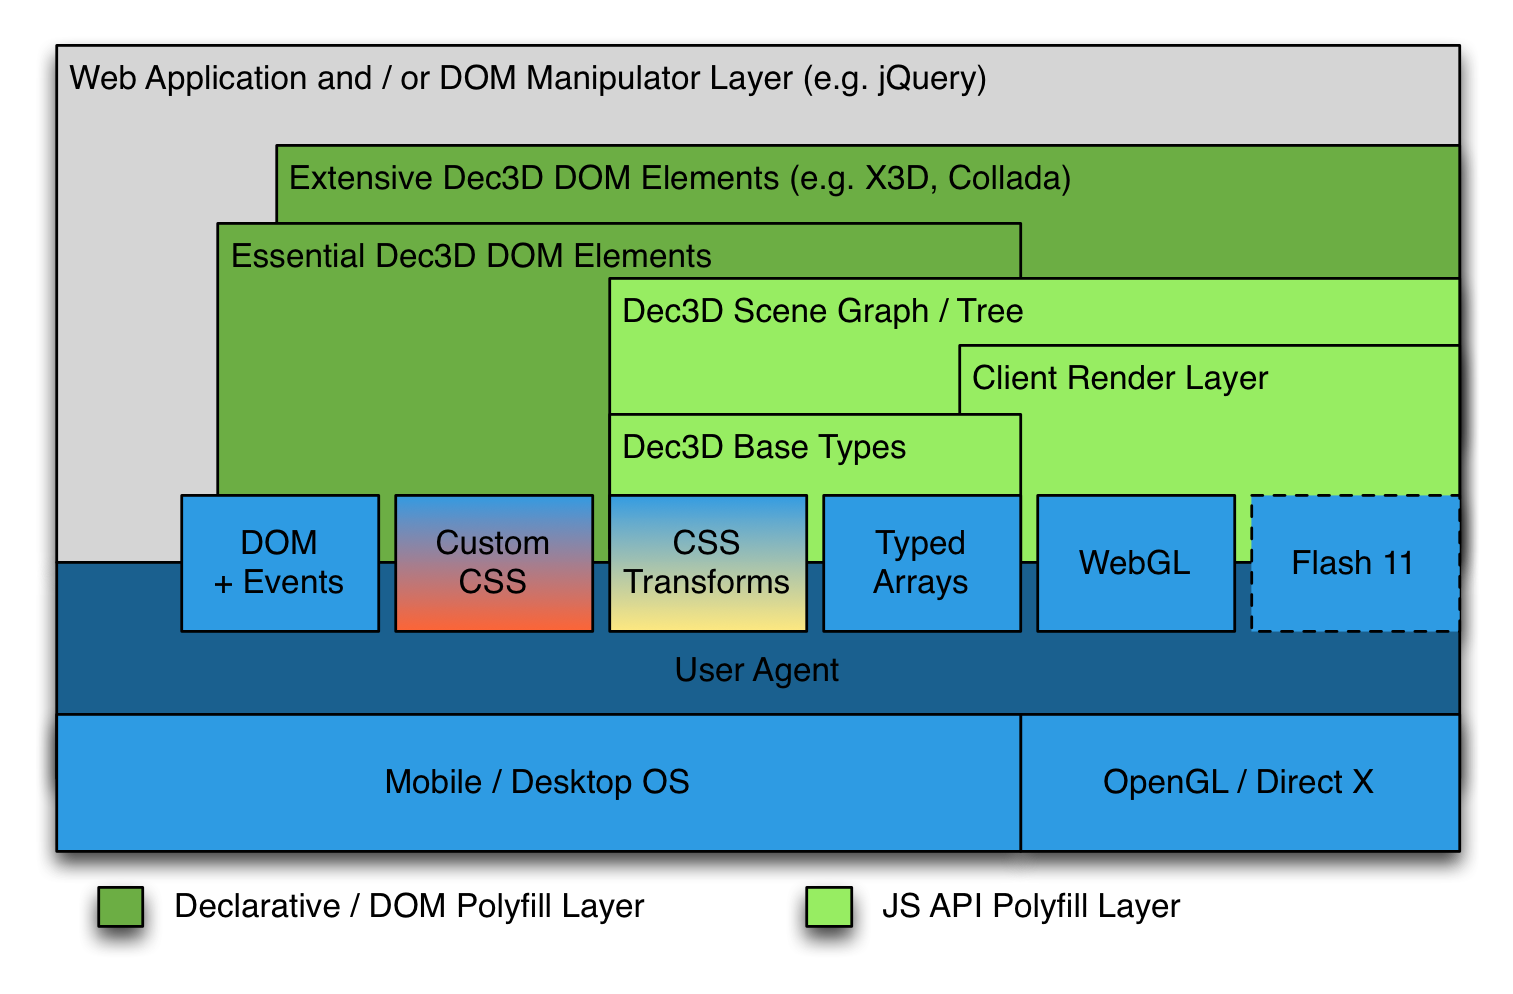
\includegraphics[width=1.0\columnwidth]{images/Dec3D-Architecture.png}
  \caption{Proposed declarative 3D ``polyfill'' runtime architecture.}
  \label{fig:polyArch}
  %\vspace{-0.2cm}
\end{figure}

% Don't cite this link but present the whole idea here!
% http://www.w3.org/community/declarative3d/wiki/Level_of_Integration/
We also propose to measure a level of integration for 3D graphics in terms of W3C technologies (DOM, CSS, etc.) to explain existing and possible integration levels (Figure \ref{fig:polyInt} shows that currently only level 2, DOM integration, is possible), and to finally identify a suitable integration level for declarative 3D. However, the latter imposes several problems in that it requires having a set of 3D-specific CSS properties or even a full shader description via CSS as well as a deeper integration into debugging tools like Chrome Developer Tools or Firebug. However, integration levels 3 and 4 are currently not yet achievable by a JavaScript implementation, because the required APIs are missing: it is not possible to introduce new CSS properties or to extend developer tools by an API.

It quickly became clear that a higher level of integration requires additional APIs in user agents. After discussions with browser vendors (namely Firefox and Chrome), who made it clear that integration of the desired extensions natively into their frameworks is not currently their priority, we decided to consider a polyfill approach for the further development activities.
Nevertheless, communicating and requesting additional and missing features like custom CSS properties or CSS monitoring is necessary.

A \textit{polyfill} is a downloadable piece of code, which provides facilities that are not natively built-in to a Web browser \cite{Sharp2010}. For example, many features of HTML5 are not supported by versions of Internet Explorer older than version 8 or 9, but can be used by web pages if those pages install a so-called polyfill. Polyfills can also be used to add entirely new functionality to browsers.

\begin{figure}
  \centering
  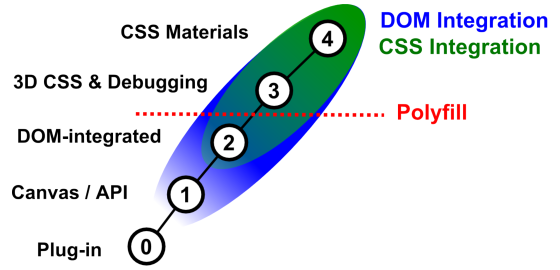
\includegraphics[width=0.85\columnwidth]{images/polyfill.png}
  \caption{Levels of integration: current browser APIs only allow integrating with DOM and DOM Events, but not yet fully with CSS.}
  \label{fig:polyInt}
  %\vspace{-0.2cm}
\end{figure}

Polyfill-based approaches allow deriving hard requirements for related and utilized W3C standards and user agent (UA) APIs immediately. This leads to much more evolving concepts and solutions in contrast to an overall declarative 3D specification. In the following we hence list our most important UA requirements.

\begin{description}
\item[DOM] The polyfill layer must be able to access and monitor changes in related DOM elements. This can be achieved using the now deprecated DOM Mutation Events as well as the new \emph{MutationObserver}\footnote{\url{https://dvcs.w3.org/hg/domcore/raw-file/tip/Overview.html\#mutation-observers}} objects.
\item[Events] The UA must support registration, firing, and extending UI events. This is mainly done through dynamic property changes in the JavaScript object, which currently represent the event for performance reasons.
\item[Custom CSS properties] The goal is to support scene management though custom CSS properties. Unfortunately, this was not possible in the last years, but may change with the new CSS Custom Properties specification \cite{CSSCustom}.
\item[CSS 3D Transforms] The CSS 3D Transforms module \cite{webkit3DCSS} is now supported in all major browsers, but the methods to monitor final matrix changes are limited right now and should be further extended for optimal performance.
\item[TypedArrays] TypedArrays \cite{TypArr12} were first introduced with the WebGL specification but are now an established method to process large portions of typed data efficiently.
\item[Generic GPU access] For client-side rendering the polyfill layer has to access the GPU functionality almost directly. Here, WebGL is there a perfect candidate and Flash 11/Stage3D a second fallback option.
\end{description}

To sum up, the X3DOM and XML3D experimental declarative 3D Web publishing frameworks are designed to explore different options for adding 3D graphics to HTML. Here, Figure \ref{fig:polyArch} depicts our proposed declarative 3D polyfill runtime architecture, though we'd like to stress that the whole integration model is still evolving and open for discussion.

\begin{figure*}
  \centering
  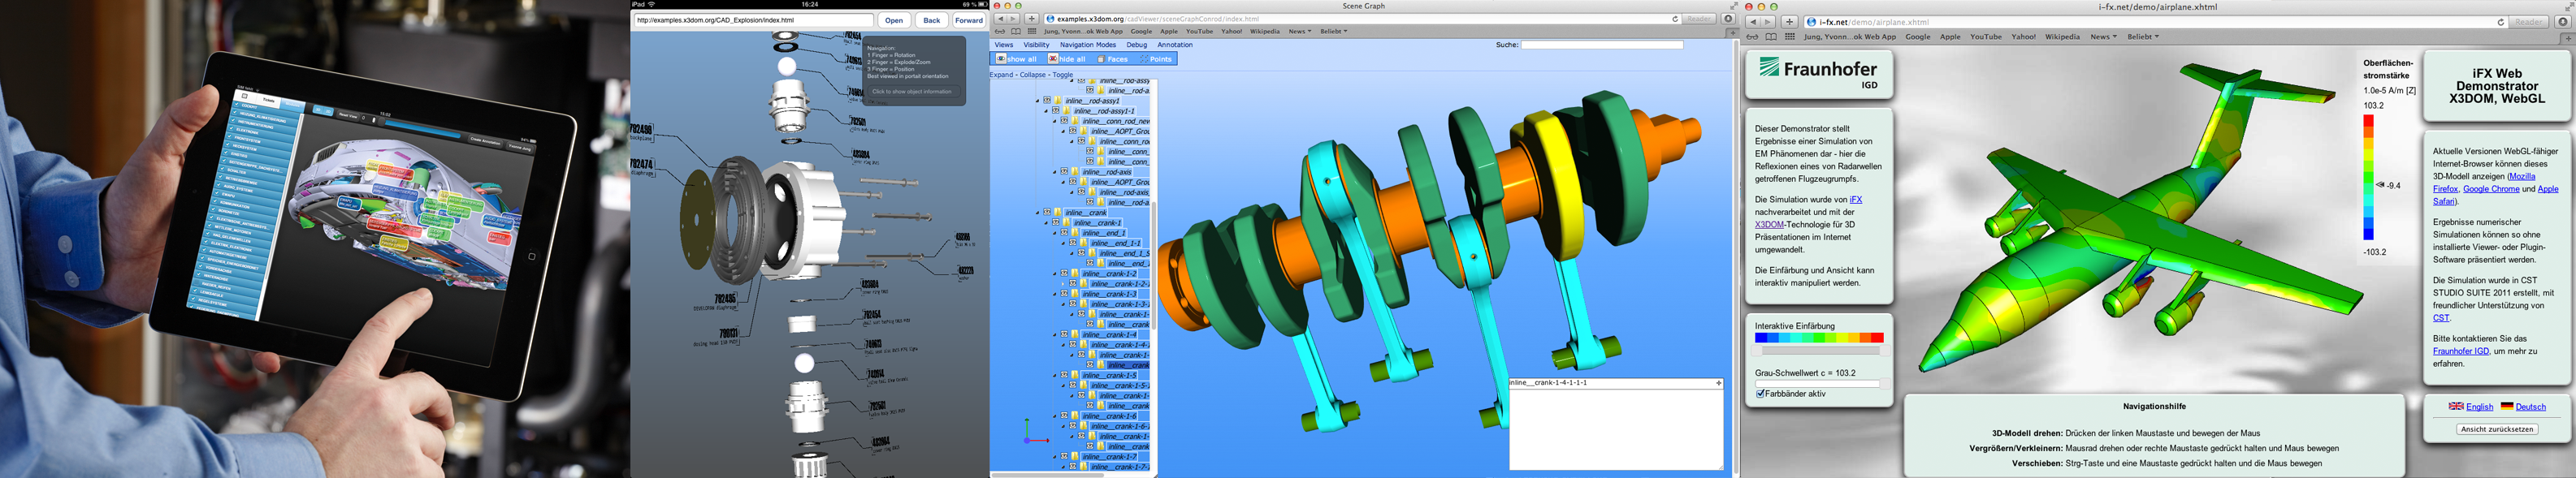
\includegraphics[width=1.0\textwidth]{images/cad_apps.png}
  \caption{From left to right: web-based design review application with annotation markers; interactive explosion of CAD model on iPad; lightweight web-based viewer for 3D CAD data; visualization and interactive exploration of simulation data by using extended mouse events.}
  \label{fig:cadApps}
  %\vspace{-0.2cm}
\end{figure*}




\section{Declarative 3D Agenda}
\label{sec:Agenda}

In this section we shape the agenda and identify upcoming research issues for the next development stage of Dec3D.
During the 1\textsuperscript{st} Intl. Workshop on Declarative 3D \cite{Dec3D2012} as well as during more informal meetings at Web3D and SIGGRAPH in 2011/2012, the members and supporters of the Declarative 3D W3C Community Group agreed upon the following topics to make the effort successful and for the W3C to adopt/develop a Dec3D standard.

\paragraph{Encourage Participation}
All relevant stakeholders, e.g. developers, designers, researchers, 3D artists, industry professionals, representatives of standards organizations, accessibility experts, and user-agent implementers, are encouraged to participate in this group. Participants should be willing to actively develop and donate materials towards the group's deliverables, as well as attend the group's teleconferences and face-to-face meetings.

\paragraph{Clear Definition of Use Cases and Requirements}
The group needs to agree on a collection of use cases, where embedding 3D data in HTML using a declarative approach provides significant benefit. Here, declarative approaches esp. seem relevant for the industry, since they tend to think in formats not in APIs.
Each use case should explore how publishers and consumers benefit from Dec3D. From these use cases, the group needs to derive and prioritize the different required dimensions for the Dec3D technical specification \cite{JankowskiDec3D2012,LeFeuvreDec3D2012}.

\paragraph{Clear Technical Specification}
The next step is the creation of the clear, detailed and extensible technical specification of the implementation concepts and features necessary to cover a majority of useful requirements. Measurable properties need to be defined to quantitatively and/or qualitatively evaluate the achieved solution, document the pros and cons of each, and demonstrate that, based on the above analysis, there is a good chance of success in creating a W3C standard for Declarative 3D for the Web.

\paragraph{Outreach and Exemplar Applications}
The group needs to continue its outreach activities through the high quality demonstrations of the Declarative 3D philosophy using the open-source frameworks X3DOM and XML3D. Therefore, several applications should be identified, each requiring and demonstrating different capabilities of Dec3D. For example, one application could require huge 3D datasets which are impractical for inclusion directly into the DOM; another could require real-time control of an external system (inter-process communication); another could integrate with a complex data base; another an illustration of complex data (information visualization) without a physical analog, and another a more traditional scientific visualization. Key to selection of these applications is the use and demonstration of a declarative 3D requirement.

\paragraph{W3C Working Group Proposal}
Finally, the Community Group should deliver reports documenting its progress, any conclusions it arrived at with respect to the standardization of \textit{Declarative 3D for the Web} and, if reaching a positive conclusion, recommending a standardization approach as a basis for a future W3C working group on the same topic.


\section{Conclusions}
\label{sec:Conclusions}

While WebGL, a 3D imperative graphics API in the Web context, is getting more and more traction, we are still missing an easy way to add interactive high-level declarative 3D objects to an HTML document to allow anyone to easily create, share, and experience interactive 3D graphics, with possibly wide ranging effects similar to those caused by the broad availability of video on the Web.
The main motivation is thus to make it easy to add 3D to Web pages by bringing 3D to the Web developers and not vice versa. This can be achieved by fully integrating 3D content into HTML5 documents, where interactive 3D graphics is a first class DOM objects. Moreover, by reusing existing Web technology wherever possible, no new concepts are added unless absolutely necessary.

Another objective of this position paper on Declarative 3D for the Web is to evaluate the options for a successful standardization of a declarative approach to interactive 3D graphics as part of HTML documents. The idea is to collect suitable use cases, derive requirements from them, and then find the essential set of features and concepts that enables broad uptake by authors and users of interactive 3D on the Web.
We are absolutely aware that our goal is ambitious and it will take some time to implement these features. Therefore, we call for more participation from the Web3D and W3C communities that we believe is crucial to achieve our common and ultimate goal: 3D for everyone and everywhere.


%\section*{Acknowledgements}

\bibliographystyle{acmsiggraph}
%\parskip3pt
\bibliography{bibliography}

\end{document}
